\chapter{Seperating Axis Theorem}

\section{Zasada działania}
Separating Axis Theorem, w skrócie SAT, jest metodą pozwalającą wykryć, czy dane dwa wielokąty wypukłe przecinają się. Odpowiednie rozwinięcie algorytmu umożliwia również znalazienie najmniejszego wektora przeniknięcia obiektów.  SAT jest algorytmem genetycznym, który pozwala szybko zweryfikować, czy nastąpiła kolizja między obiektami. Niweluje to konieczność stosowania złożonych obliczeniowo jak i czasowo algorytmów, umożliwiając sprawdzenie kolizji dla duzej liczby obiektów bez spadku wydajności aplikacji.\\
Ogólna zasada działania Separating Axis Theorem polega na sprawdzeniu, czy istnieje oś dzieląca sprawdzane obiekty bez ich przecinania. Jeśli nie jest możliwe znalezienie takiej osi, oznacza to, iż zaistniała kolizja tych obiektów. Teoretycznie itsnieje nieskończenie wiele osi, które możemy sprawdzić. W praktyce wystarczy sprawdzić jedynie osie wzdłuż normalnych płaszczyzn, z których składają się obiekty oraz wzdłuż osi stworzonych z iloczynów wektorowych brzegów obiektów. Jeśli wzdłuż choćby jednej z sprawdzanych osi obiekty nie przecinają się, oznacza to, że istnieje oś dzieląca sprawdzane obiekty, więc kolizja nie występuje. Dla sześcianu będzie to sprawdzenie 3 osi wzdłuż normalnych płaszczyzn obiektu (łącznie sześć osi) oraz iloczynu wektorowego osi wzdłuż brzegów (dziewięć osi). \\

\section{Iloczyn wektorowy}
Wynikiem iloczynu wektorowego nowy wektor o kierunku prostopadłym do płaszczyzny utworzonej przez mnożone wektory o długości równej iloczynowi długosci wektorów oraz sinusa kąta między nimi. Zwrot utworzonego wektora wyznaczany jest regułą prawej ręki lub regułą śruby prawoskrętnej.Kolejność mnożenia odgrywa tu niemałe znaczenie,ponieważ wynik iloczynu wektorowego AxB nie równa się BxA. \\ \\
Wartość iloczynu wektorowego zdefiniowana jest następujacym wzorem: \\
\centering
$|\vec{a} \times \vec{b}|= |\vec{a}| \bullet |\vec{b}| \bullet \sin\gamma$
\flushleft
%\begin{figure}[h]
%\centering
%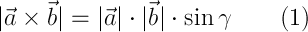
\includegraphics[width=0.3\textwidth]{figures/iloczyn1.png}
%\end{figure}
Produkt iloczynu skalarnego wektorów a i b ma postać: \\
\centering$a \times b = \vec{a} \times \vec{b} = $\\
%\begin{figure}[h]
%\centering
%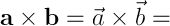
\includegraphics[width=0.2\textwidth]{figures/iloczyn2.png}
%\end{figure} 
$= (a_{x} b_{z} - a_{z} b_{y})\widehat{x} +  (a_{z} b_{x} - a_{x} b_{z})\widehat{y} +  (a_{x} b_{y} - a_{y} b_{y})\widehat{z}$\\\flushleft
%\begin{figure}[h]
%\centering
%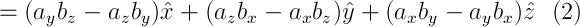
\includegraphics[width=0.8\textwidth]{figures/iloczyn21.png}
%\end{figure} 
co równoważne jest z zapisem: \\
\centering
$ \vec{a} \times \vec{b} = [a_{x} b_{z} - a_{z} b_{y}, a_{z} b_{x} - a_{x} b_{z}, a_{x} b_{y} - a_{y} b_{y}]$
\flushleft
%\begin{figure}[h]
%\centering
%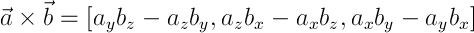
\includegraphics[width=0.4\textwidth]{figures/iloczyn22.png}
%\end{figure} 